\documentclass[12pt]{extarticle}
\usepackage{amsmath}
\usepackage{tikz}
\usepackage{verbatim}
\usepackage{amsfonts}
\usepackage{amssymb}
\usepackage{graphicx}
\usepackage{mathtools}
\usepackage{color}
\usepackage{hyperref}
\usepackage[utf8]{inputenc}
\usepackage[margin=0.5in]{geometry}
\newcommand\tab[1][1cm]{\hspace*{#1}}
\usepackage{collectbox}
\DeclarePairedDelimiter\ceil{\lceils}{\rceil}
\DeclarePairedDelimiter\floor{\lfloor}{\rfloor}
\usepackage{amsthm}
%opening
\title{Software Compilation}
\author{Daniel Drake}

\theoremstyle{plain}
\newtheorem{thm}{Theorem}[section] 

\theoremstyle{plain}
\newtheorem{axiom}{Axiom}[section] 

\theoremstyle{plain}
\newtheorem{lma}{Lemma}[section] 

\theoremstyle{Definition}
\newtheorem{def.}{Definition}[section] 

\theoremstyle{Definition}
\newtheorem{prf}{Proof}[section] 

\theoremstyle{plain}
\newtheorem{exmp}{Example}[section]

\theoremstyle{plain}
\newtheorem{ruleOfInference}{Rule Of Inference}[section]

\newcommand{\cut}[0]{\noindent\framebox[\linewidth]{\rule{\linewidth}{2pt}}\\}
\newcommand{\prof}[0]{	\noindent \textbf{Proof:} \rule{500pt}{2pt} \\ }

\newcommand{\ddash}{\boxed{\vdash}}

\begin{document}
	
	\section{Introduction}
		Meh, I don't like writing narratives. We are here to start with turning code into software. As a starting place, I will cover the basics of c++ compilation without the use of any sort of IDE. 
	\section{gcc}
		The formal description of the gcc tool is:
		\begin{quotation}
			GCC stands for “GNU Compiler Collection”. GCC is an integrated distribution of compilers for several major programming languages. These languages currently include C, C++, Objective-C, Objective-C++, Fortran, Ada, D, Go, and BRIG (HSAIL). 
		\end{quotation}
		The gcc tool is a very complex tools with all kinds of uses, most of which I won't cover here. This is ultimately unnecessary since there is this neat resource with has been written by the people who maintain this tool. Here is the reference: \href{https://gcc.gnu.org/onlinedocs/}{Super Awesome Reference}. \\
		You will need to know which version of gcc you have. To learn this simply execute: 
		\verb|gcc --version| \\
		Given these things, you should be able to figure out everything you would ever need to know about gcc. \\
		To cover some basic usage of this command, I will demonstrate it's use. \\ \\
	\textbf{Example: Oh, that’s Wow, Morty. Wow. What an exciting life you lead. Let’s go. In and out, 20 minutes adventure. } \\ \\
		Given a directory structure like so: \\ 
		\begin{center}	
			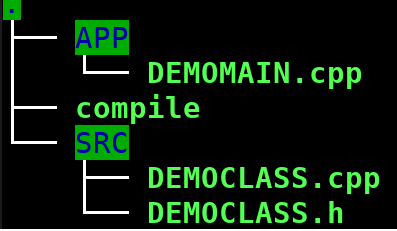
\includegraphics{demo.png}			
		\end{center}		
	Then our compile script holds the simple command:
	\begin{center}
		\verb|gcc -x c++ APP/DEMOMAIN.cpp SRC/DEMOCLASS.h SRC/DEMOCLASS.cpp -o DEMOEXE -lstdc++|
	\end{center}
	Lets look at this command. The -x option allows us to select the language for the following input files
(rather than letting the compiler choose a default based on the
	file name suffix). This is necessary as by default, the gcc tool will treat all files as c files. Next we have n paths to different source files. In this case we have 3. Next we have the -o flag which allows us to name the executable file. Finally, since the stdc++ library isn't linked to by default with the gcc compile, we have to state it explicitly. 
	With all that out of the way, if the compile file has executable permission, then we can run it to compile the files. 

	\section{Includes}
		When compiling a program using the \verb|-v| we can see things like where the compiler is looking to find libraries that you might link to. Adding the option \verb|-Wl,--trace| to the end of the gcc command will tell you where the libraries are which you are linking to. 
	\section{Make}
		Next, we come to make files. \\
		Makefiles are like my compile script, however it's a standardized way for handling larger systems of code. Once again we are playing with a pretty complicated tool here however it also has a great reference maintained by the people who maintain the make tool. Here is the reference: \href{https://www.gnu.org/software/make/manual/make.html}{Dank Reference Time} \\
		So to use a Makefile, generally what you would call is just: \verb|make| while in a directory containing a file called Makefile. This will create an compile command like I demonstrated earlier and execute it. \\
		Next up is a demo of a Makefile which lives in the same directory as our compile script though totally independent of that script. \\ \\
		\textbf{Example: Yo, I heard you like compilation automation.} 
		\verbatiminput{/home/drake/DSYS/DDEMO/DMAKEDEMO/DEMO0/Makefile}
		Here, both FLAGS and LIBS are called macros and are not themselves executed. They are variables you can set and call using the \verb|$(VAR)| syntax. \\ 
		The \verb|all| tag is the first target and therefore the default target. \\ 
		The general syntax for targets is: \\ 
		\verb|target: prerequisites| \\
		\verb|<TAB> recipe| \\
		The tab is necessary, latex just didn't want to add that information with how I am linking the file. 
		One great advantage of handling the compilation this way is that if a file changes, make will only rebuild that part of the system and not the entire thing. This doesn't matter when dealing with smaller problems but is extremely helpful when dealing with larger projects. 
		Each of these targets can be called individually by using the following syntax: \\
		\verb|make target1 target2 ... targetN| \\
		However if just make is called then it will run the default target. 
	\section{CMake}
		This is great and all, but what if you didn't want to generate the makefile yourself and instead wanted a way to just list the files and libraries you want to use and have the Makefile generated for you? Here comes cmake with the cure for what ails you. Cmake is another tool which is very complex and with our complex tools comes a sweet reference you can use to learn all kinds of stuff about it: \href{https://cmake.org/documentation/}{Sweet Reference Time}. 
		We are here for demonstrations however and so here we go. \\ \\
		\textbf{Example 1: I put some automation in your automation so you can automate while you automate.} \\ \\
		For this you will need a file called: \verb|CMakeLists.txt| in the same directory as the other compilation files. 
		\verbatiminput{/home/drake/DSYS/DDEMO/DMAKEDEMO/DEMO0/CMakeLists.txt}
		The whitespace format is messed up again here. \\
		Calling \verb|cmake .| here will generate everything needed to build the project. \\ 
		After that you can call \verb|make| and it will generate the executable. 
		This is a much simpler file format and can be expanded to reference other libraries needed. \\ \\
		\textbf{Example 2: Return of the King} \\ \\
		This is an actual example which I am currently using to build all the source code for my main project DSYS. 
		\verbatiminput{/home/drake/DSYS/CMakeLists.txt}


\end{document}